\documentclass{beamer}

\usepackage{fontspec}
\usepackage{subcaption}
\newfontfamily{\unicodefont}{Cambria}

\setbeamertemplate{caption}[numbered]


\mode<presentation>
{
	\usetheme{CambridgeUS}
	
	\setbeamercovered{transparent}
	% or whatever (possibly just delete it)
}

\title[CAN304 Group 16 Presentation]
{TrueSeeing: Defensive software against text-encoding based invisible attacks}

\author[Group 16]
{%
	Chunyu Jiang \and
	Guanyuming He \and
	Hanyu Zhang \and
	Kemu Xu \and
	Yifei Du \and
	Yilu Shi%
}

\subtitle
{CAN304 Group 16 Presentation}

\institute[XJTLU]
{
	Department of Computing, School of Advanced Technology\\
	Xi'an Jiaotong-Liverpool University%
}

\date
{21 May, 2024 / SC169}

\pgfdeclareimage[height=0.5cm]{university-logo}{./assets/university_logo.png}
\logo{\pgfuseimage{university-logo}}

\begin{document}
	
\begin{frame}
	\titlepage
\end{frame}

%\begin{frame}{Contents}
%	\tableofcontents
%\end{frame}

\begin{frame}{Introduction:\\Do these two words look the same to you?}
\begin{columns}
	\Large
	\column{.5\textwidth}
	{\unicodefont United states}
	
	\column{.5\textwidth}
	{\unicodefont Un\symbol{"456}ted \symbol{"0455}t\symbol{"430}tes}
\end{columns}
\end{frame}

\begin{frame}{This happens because...}
\begin{itemize}
	\item Texts, like all other digital data, are stored in binary.
	\item We humans see texts visually.
	\item But some programs, like ChatGPT, compilers, search engines, see them in binary.
	\item And there are many ways to make texts that look the same but different in binary.
\end{itemize}
\end{frame}

\begin{frame}{State-of-the-art attack methods}
\begin{description}
	\item[Invisible Characters] You cannot see some characters that a program can see.
	\item[Homoglyphs] Different characters that look the same (the introduction).
	\item[Reordering] Texts whose order looks different to you and to a computer program.
	\item[Deleteion] Something you can see cannot be seen by a computer program.
\end{description}
\end{frame}

\begin{frame}{How to stop this...}
	\begin{itemize}
		\item Make the programs see as you see (hard).
		\item Make you see the evil binary characters (easy).
		\item And remove them.
	\end{itemize}
\end{frame}

\begin{frame}{Therefore we present TrueSeeing}
	\begin{itemize}
	\item It accepts texts from clipboard and files.
	\item It renders them in two ways simultaneously:
		\begin{enumerate}
		\item What you would normally see.
		\item Expose all the evil characters.
		\end{enumerate}
	\item Then you are allowed to make modifications to the text until all evil characters are gone.
	\end{itemize}
\end{frame}

\begin{frame}{Prevent the text from being exploited again}
	TrueSeeing also allows you to give a digital signature to the neutralised text: RSA-FDH
        \begin{itemize}
	      \item Gen: RSAGen: public key $(N, e)$, private key $(N, d)$
	      \item Sign: $\sigma = H(m)^d \bmod N$
            \item Vrfy: \[ Vrfy_{pk}(m, \sigma) = 
                \begin{cases} 
                    1, & \text{if } \sigma^e = H(m) \bmod N \\
                    0, & \text{otherwise}
                \end{cases}
                \]
	\end{itemize}
\end{frame}

\begin{frame}{Demonstration: TrueSeeing - Encoding Format}
\begin{columns}
    \begin{column}{.6\textwidth}
        \centering
        Choose Encoding format
        
        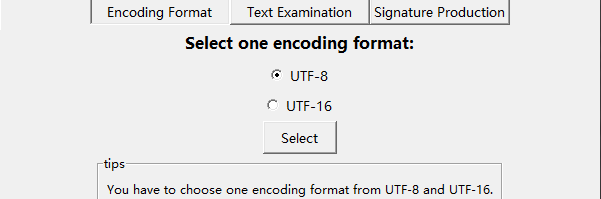
\includegraphics[width=.8\columnwidth]{assets/Encode.png}

        Revealing Malicious Characters
        
        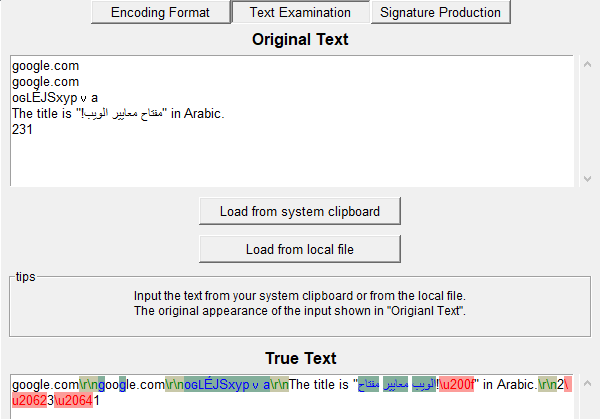
\includegraphics[width=.8\columnwidth]{assets/text.png}
    \end{column}
    
    \begin{column}{.5\textwidth}
        \centering
        Digital Signature

		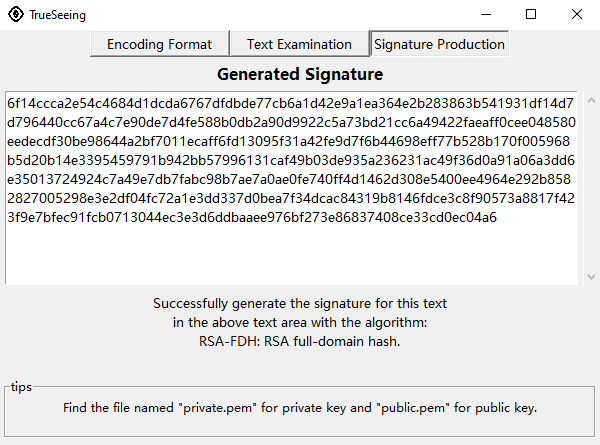
\includegraphics[width=\columnwidth]{assets/signature.png}
    \end{column}
\end{columns}
\end{frame}


\begin{frame}{Thank You}
\begin{center}
	\Huge Feel free to ask Questions.
\end{center}
\end{frame}
	
\end{document}